\hypertarget{transport-design}{}\section{JACK Transport Design}\label{transport-design}
The \hyperlink{index_index}{JACK Audio Connection Kit} provides simple transport interfaces for starting, stopping and repositioning a set of clients. This document describes the overall design of these interfaces, their detailed specifications are in $<$jack/transport.h$>$

\begin{itemize}
\item \hyperlink{transport-design_requirements}{Requirements}\item \hyperlink{transport-design_overview}{Overview}\item \hyperlink{transport-design_timebase}{Timebase Master}\item \hyperlink{transport-design_transportcontrol}{Transport Control}\item \hyperlink{transport-design_transportclients}{Transport Clients}\item \hyperlink{transport-design_compatibility}{Compatibility}\item \hyperlink{transport-design_issues}{Issues Not Addressed}\end{itemize}
\hypertarget{transport-design_requirements}{}\subsection{Requirements}\label{transport-design_requirements}
\begin{itemize}
\item We need sample-level accuracy for transport control. This implies that the transport client logic has to be part of the realtime process chain.\end{itemize}


\begin{itemize}
\item We don't want to add another context switch. So, the transport client logic has to run in the context of the client's process thread. To avoid making an extra pass through the process graph, no transport changes take effect until the following process cycle. That way, the transport info is stable throughout each cycle.\end{itemize}


\begin{itemize}
\item We want to allow multiple clients to change the transport state. This is mostly a usability issue. Any client can start or stop playback, or seek to a new location. The user need not switch windows to accomplish these tasks.\end{itemize}


\begin{itemize}
\item We want a way for clients with heavyweight state to sync up when the user presses \char`\"{}play\char`\"{}, before the transport starts rolling.\end{itemize}


\begin{itemize}
\item We want to provide for ongoing binary compatibility as the transport design evolves.\end{itemize}
\hypertarget{transport-design_overview}{}\subsection{Overview}\label{transport-design_overview}
The former transport master role has been divided into two layers:

\begin{itemize}
\item \hyperlink{transport-design_timebase}{Timebase Master} - counting beats, frames, etc. on every cycle.\item \hyperlink{transport-design_transportcontrol}{Transport Control} - start, stop and reposition the playback.\end{itemize}


Existing transport clients continue to work in compatibility mode. But, old-style timebase masters will no longer control the transport.\hypertarget{transport-design_timebase}{}\subsection{Timebase Master}\label{transport-design_timebase}
The timebase master continuously updates extended position information, counting beats, timecode, etc. Without this extended information, there is no need for this function. There is at most one master active at a time. If no client is registered as timebase master, frame numbers will be the only position information available.

The timebase master registers a callback that updates position information while the transport is rolling. Its output affects the following process cycle. This function is called immediately after the process callback in the same thread whenever the transport is rolling, or when any client has set a new position in the previous cycle. The first cycle after \hyperlink{transport_8h_d1d237a74417e8b4a4bc7894afefc1cb}{jack\_\-set\_\-timebase\_\-callback()} is also treated as a new position, or the first cycle after \hyperlink{jack_8h_c7dc9d6132b8331ab500cdb593b8de11}{jack\_\-activate()} if the client had been inactive.



\footnotesize\begin{verbatim}  typedef int  (*JackTimebaseCallback)(jack_transport_state_t state,
                                       jack_nframes_t nframes,
                                       jack_position_t *pos,
                                       int new_pos,
                                       void *arg);
\end{verbatim}
\normalsize


When a new client takes over, the former timebase callback is no longer called. Taking over the timebase may be done conditionally, in which case the takeover fails when there is a master already. The existing master can release it voluntarily, if desired.



\footnotesize\begin{verbatim}  int  jack_set_timebase_callback (jack_client_t *client,
                                   int conditional,
                                   JackTimebaseCallback timebase_callback,
                                   void *arg);

  int  jack_release_timebase(jack_client_t *client);
\end{verbatim}
\normalsize


If the timebase master releases the timebase or exits the JACK graph for any reason, the JACK engine takes over at the start of the next process cycle. The transport state does not change. If rolling, it continues to play, with frame numbers as the only available position information.\hypertarget{transport-design_transportcontrol}{}\subsection{Transport Control}\label{transport-design_transportcontrol}
The JACK engine itself manages stopping and starting of the transport. Any client can make transport control requests at any time. These requests take effect no sooner than the next process cycle, sometimes later. The transport state is always valid, initially it is \hyperlink{transport_8h_499ffea77b03cce9c647d7b5065f733866566fe3891dbba7d3cdda2b7fef1793}{Jack\-Transport\-Stopped}.



\footnotesize\begin{verbatim}  void jack_transport_start (jack_client_t *client);
  void jack_transport_stop (jack_client_t *client);
\end{verbatim}
\normalsize


The engine handles polling of slow-sync clients. When someone calls \hyperlink{transport_8h_6c868184c830c2e84b7ea4d04ab1aba9}{jack\_\-transport\_\-start()}, the engine resets the poll bits and changes to a new state, \hyperlink{transport_8h_499ffea77b03cce9c647d7b5065f733826f99f6e435fe2f37ffce708fe128d12}{Jack\-Transport\-Starting}. The {\em sync\_\-callback\/} function for each slow-sync client will be invoked in the JACK process thread while the transport is starting. If it has not already done so, the client needs to initiate a seek to reach the starting position. The {\em sync\_\-callback\/} returns false until the seek completes and the client is ready to play. When all slow-sync clients are ready, the state changes to \hyperlink{transport_8h_499ffea77b03cce9c647d7b5065f733807b572e2dbc92cf006e07cc23befaece}{Jack\-Transport\-Rolling}.



\footnotesize\begin{verbatim}  typedef int  (*JackSyncCallback)(jack_transport_state_t state,
                                   jack_position_t *pos, void *arg);
\end{verbatim}
\normalsize


This callback is a realtime function that runs in the JACK process thread.



\footnotesize\begin{verbatim}  int  jack_set_sync_callback (jack_client_t *client,
                               JackSyncCallback sync_callback, void *arg);
\end{verbatim}
\normalsize


Clients that don't declare a {\em sync\_\-callback\/} are assumed to be ready immediately, any time the transport wants to start. If a client no longer requires slow-sync processing, it can set its {\em sync\_\-callback\/} to NULL.



\footnotesize\begin{verbatim}  int  jack_set_sync_timeout (jack_client_t *client,
                              jack_time_t usecs);
\end{verbatim}
\normalsize


There must be a {\em timeout\/} to prevent unresponsive slow-sync clients from completely halting the transport mechanism. Two seconds is the default. When this {\em timeout\/} expires, the transport will start rolling, even if some slow-sync clients are still unready. The {\em sync\_\-callback\/} for these clients continues being invoked, giving them an opportunity to catch up.



\footnotesize\begin{verbatim}  int  jack_transport_reposition (jack_client_t *client,
                                  jack_position_t *pos);
  int  jack_transport_locate (jack_client_t *client,
                              jack_nframes_t frame);
\end{verbatim}
\normalsize


These request a new transport position. They can be called at any time by any client. Even the timebase master must use them. If the request is valid, it goes into effect in two process cycles. If there are slow-sync clients and the transport is already rolling, it will enter the \hyperlink{transport_8h_499ffea77b03cce9c647d7b5065f733826f99f6e435fe2f37ffce708fe128d12}{Jack\-Transport\-Starting} state and begin invoking their {\em sync\_\-callbacks\/} until ready.

\begin{figure}[H]
\begin{center}
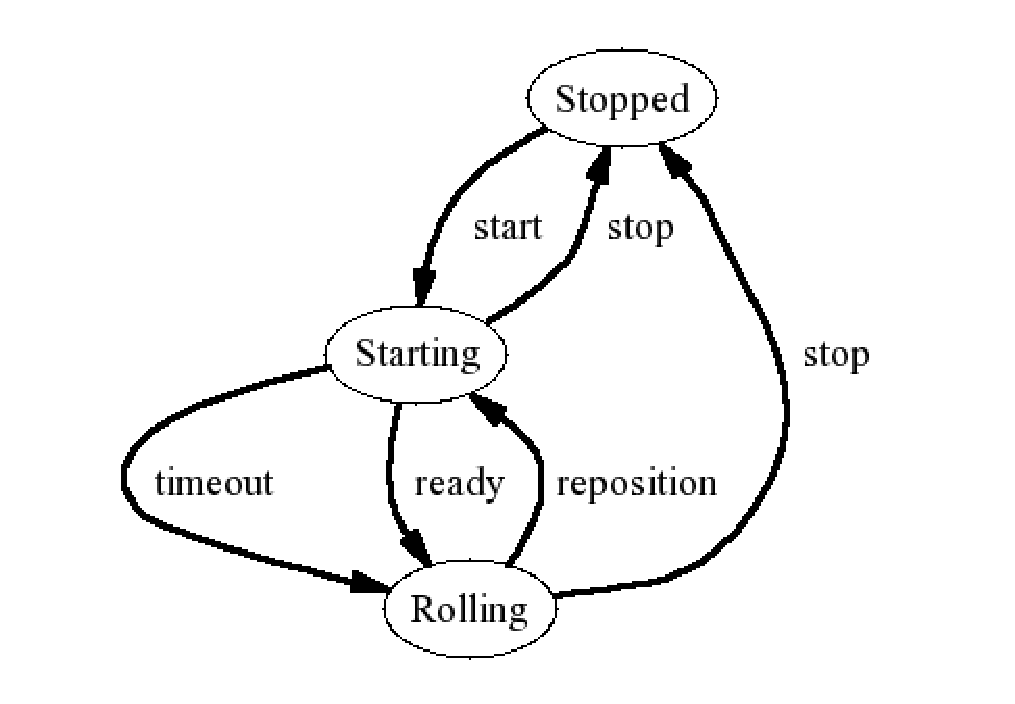
\includegraphics{fsm}\caption{Transport State Transition Diagram}
\end{center}
\end{figure}
\hypertarget{transport-design_transportclients}{}\subsection{Transport Clients}\label{transport-design_transportclients}
Transport clients were formerly known as \char`\"{}transport slaves\char`\"{}. We want to make it easy for almost every JACK client to be a transport client.



\footnotesize\begin{verbatim}   jack_transport_state_t jack_transport_query (jack_client_t *client,
                                                jack_position_t *pos);
\end{verbatim}
\normalsize


This function can be called from any thread. If called from the process thread, {\em pos\/} corresponds to the first frame of the current cycle and the state returned is valid for the entire cycle.\hypertarget{transport-design_compatibility}{}\subsection{Compatibility}\label{transport-design_compatibility}
During the transition period we will support the old-style interfaces in compatibility mode as deprecated interfaces. This compatibility is not 100\%, there are limitations.

The main reasons for doing this are:

\begin{itemize}
\item facilitate testing with clients that already have transport support\item provide a clean migration path, so application developers are not discouraged from supporting the transport interface\end{itemize}


These deprecated interfaces continue to work:



\footnotesize\begin{verbatim}  typedef struct jack_transport_info_t;

  void jack_get_transport_info (jack_client_t *client,
                                jack_transport_info_t *tinfo);
\end{verbatim}
\normalsize


Unfortunately, the old-style timebase master interface cannot coexist cleanly with such new features as \hyperlink{transport_8h_683f8877d18010277fd4e1b0b658e075}{jack\_\-transport\_\-locate()} and slow-sync clients. So, these interfaces are only present as stubs:



\footnotesize\begin{verbatim}  void jack_set_transport_info (jack_client_t *client,
                                jack_transport_info_t *tinfo);
  int  jack_engine_takeover_timebase (jack_client_t *);
\end{verbatim}
\normalsize


For compatibility with future changes, it would be good to avoid structures entirely. Nevertheless, the \hyperlink{structjack__position__t}{jack\_\-position\_\-t} structure provides a convenient way to collect timebase information in several formats that clearly all refer to a single moment. To minimize future binary compatibility problems, this structure has some padding at the end, making it possible to extend it without necessarily breaking compatibility. New fields can be allocated from the padding area, with access controlled by newly defined valid bits, all of which are currently forced to zero. That allows the structure size and offsets to remain constant.\hypertarget{transport-design_issues}{}\subsection{Issues Not Addressed}\label{transport-design_issues}
This design currently does not address several issues. This means they will probably not be included in JACK release 1.0.

\begin{itemize}
\item variable speed\item reverse play\item looping \end{itemize}
